% Options for packages loaded elsewhere
\PassOptionsToPackage{unicode}{hyperref}
\PassOptionsToPackage{hyphens}{url}
%
\documentclass[
  12pt,
  a4paper,
]{scrreprt}
\usepackage{amsmath,amssymb}
\usepackage{setspace}
\usepackage{iftex}
\ifPDFTeX
  \usepackage[T1]{fontenc}
  \usepackage[utf8]{inputenc}
  \usepackage{textcomp} % provide euro and other symbols
\else % if luatex or xetex
  \usepackage{unicode-math} % this also loads fontspec
  \defaultfontfeatures{Scale=MatchLowercase}
  \defaultfontfeatures[\rmfamily]{Ligatures=TeX,Scale=1}
\fi
\usepackage{lmodern}
\ifPDFTeX\else
  % xetex/luatex font selection
  \setmainfont[Ligatures=TeX]{PT Serif}
  \setsansfont[Ligatures=TeX,Scale=MatchLowercase]{PT Sans}
  \setmonofont[Scale=MatchLowercase,Scale=0.9]{PT Mono}
\fi
% Use upquote if available, for straight quotes in verbatim environments
\IfFileExists{upquote.sty}{\usepackage{upquote}}{}
\IfFileExists{microtype.sty}{% use microtype if available
  \usepackage[]{microtype}
  \UseMicrotypeSet[protrusion]{basicmath} % disable protrusion for tt fonts
}{}
\usepackage{xcolor}
\usepackage{longtable,booktabs,array}
\usepackage{calc} % for calculating minipage widths
% Correct order of tables after \paragraph or \subparagraph
\usepackage{etoolbox}
\makeatletter
\patchcmd\longtable{\par}{\if@noskipsec\mbox{}\fi\par}{}{}
\makeatother
% Allow footnotes in longtable head/foot
\IfFileExists{footnotehyper.sty}{\usepackage{footnotehyper}}{\usepackage{footnote}}
\makesavenoteenv{longtable}
\usepackage{graphicx}
\makeatletter
\def\maxwidth{\ifdim\Gin@nat@width>\linewidth\linewidth\else\Gin@nat@width\fi}
\def\maxheight{\ifdim\Gin@nat@height>\textheight\textheight\else\Gin@nat@height\fi}
\makeatother
% Scale images if necessary, so that they will not overflow the page
% margins by default, and it is still possible to overwrite the defaults
% using explicit options in \includegraphics[width, height, ...]{}
\setkeys{Gin}{width=\maxwidth,height=\maxheight,keepaspectratio}
% Set default figure placement to htbp
\makeatletter
\def\fps@figure{htbp}
\makeatother
\setlength{\emergencystretch}{3em} % prevent overfull lines
\providecommand{\tightlist}{%
  \setlength{\itemsep}{0pt}\setlength{\parskip}{0pt}}
\setcounter{secnumdepth}{5}
\newlength{\cslhangindent}
\setlength{\cslhangindent}{1.5em}
\newlength{\csllabelwidth}
\setlength{\csllabelwidth}{3em}
\newlength{\cslentryspacingunit} % times entry-spacing
\setlength{\cslentryspacingunit}{\parskip}
\newenvironment{CSLReferences}[2] % #1 hanging-ident, #2 entry spacing
 {% don't indent paragraphs
  \setlength{\parindent}{0pt}
  % turn on hanging indent if param 1 is 1
  \ifodd #1
  \let\oldpar\par
  \def\par{\hangindent=\cslhangindent\oldpar}
  \fi
  % set entry spacing
  \setlength{\parskip}{#2\cslentryspacingunit}
 }%
 {}
\usepackage{calc}
\newcommand{\CSLBlock}[1]{#1\hfill\break}
\newcommand{\CSLLeftMargin}[1]{\parbox[t]{\csllabelwidth}{#1}}
\newcommand{\CSLRightInline}[1]{\parbox[t]{\linewidth - \csllabelwidth}{#1}\break}
\newcommand{\CSLIndent}[1]{\hspace{\cslhangindent}#1}
\ifLuaTeX
\usepackage[bidi=basic]{babel}
\else
\usepackage[bidi=default]{babel}
\fi
\babelprovide[main,import]{russian}
\ifPDFTeX
\else
\babelfont[russian]{rm}{PT Serif}
\fi
\babelprovide[import]{english}
% get rid of language-specific shorthands (see #6817):
\let\LanguageShortHands\languageshorthands
\def\languageshorthands#1{}
\usepackage{indentfirst}
\usepackage{float}
\floatplacement{figure}{H}
\makeatletter
\@ifpackageloaded{subfig}{}{\usepackage{subfig}}
\@ifpackageloaded{caption}{}{\usepackage{caption}}
\captionsetup[subfloat]{margin=0.5em}
\AtBeginDocument{%
\renewcommand*\figurename{Рис.}
\renewcommand*\tablename{Таблица}
}
\AtBeginDocument{%
\renewcommand*\listfigurename{Список иллюстраций}
\renewcommand*\listtablename{Список таблиц}
}
\newcounter{pandoccrossref@subfigures@footnote@counter}
\newenvironment{pandoccrossrefsubfigures}{%
\setcounter{pandoccrossref@subfigures@footnote@counter}{0}
\begin{figure}\centering%
\gdef\global@pandoccrossref@subfigures@footnotes{}%
\DeclareRobustCommand{\footnote}[1]{\footnotemark%
\stepcounter{pandoccrossref@subfigures@footnote@counter}%
\ifx\global@pandoccrossref@subfigures@footnotes\empty%
\gdef\global@pandoccrossref@subfigures@footnotes{{##1}}%
\else%
\g@addto@macro\global@pandoccrossref@subfigures@footnotes{, {##1}}%
\fi}}%
{\end{figure}%
\addtocounter{footnote}{-\value{pandoccrossref@subfigures@footnote@counter}}
\@for\f:=\global@pandoccrossref@subfigures@footnotes\do{\stepcounter{footnote}\footnotetext{\f}}%
\gdef\global@pandoccrossref@subfigures@footnotes{}}
\@ifpackageloaded{float}{}{\usepackage{float}}
\floatstyle{ruled}
\@ifundefined{c@chapter}{\newfloat{codelisting}{h}{lop}}{\newfloat{codelisting}{h}{lop}[chapter]}
\floatname{codelisting}{Листинг}
\newcommand*\listoflistings{\listof{codelisting}{Листинги}}
\makeatother
\ifLuaTeX
  \usepackage{selnolig}  % disable illegal ligatures
\fi
\usepackage[style=gost-numeric,parentracker=true,backend=biber,hyperref=auto,language=auto,autolang=other*,citestyle=gost-numeric]{biblatex}
\addbibresource{bib/cite.bib}
\IfFileExists{bookmark.sty}{\usepackage{bookmark}}{\usepackage{hyperref}}
\IfFileExists{xurl.sty}{\usepackage{xurl}}{} % add URL line breaks if available
\urlstyle{same}
\hypersetup{
  pdftitle={Отчет по лабораторной работе 8},
  pdfauthor={Шалыгин Георгий Эдуардович},
  pdflang={ru-RU},
  hidelinks,
  pdfcreator={LaTeX via pandoc}}

\title{Отчет по лабораторной работе 8}
\usepackage{etoolbox}
\makeatletter
\providecommand{\subtitle}[1]{% add subtitle to \maketitle
  \apptocmd{\@title}{\par {\large #1 \par}}{}{}
}
\makeatother
\subtitle{Модель конкуренции двух фирм}
\author{Шалыгин Георгий Эдуардович}
\date{}

\begin{document}
\maketitle

\renewcommand*\contentsname{Содержание}
{
\setcounter{tocdepth}{2}
\tableofcontents
}
\listoffigures
\listoftables
\setstretch{1.5}
\hypertarget{ux446ux435ux43bux44c-ux440ux430ux431ux43eux442ux44b}{%
\chapter{Цель
работы}\label{ux446ux435ux43bux44c-ux440ux430ux431ux43eux442ux44b}}

Изучить построение математической модели конкуренции двух фирм .

\hypertarget{ux437ux430ux434ux430ux43dux438ux435}{%
\chapter{Задание}\label{ux437ux430ux434ux430ux43dux438ux435}}

\begin{enumerate}
\def\labelenumi{\arabic{enumi}.}
\tightlist
\item
  Постройте графики изменения оборотных средств фирмы 1 и фирмы 2 без
  учета постоянных издержек и с веденной нормировкой для случая 1.
\item
  Постройте графики изменения оборотных средств фирмы 1 и фирмы 2 без
  учета постоянных издержек и с веденной нормировкой для случая 2.
\end{enumerate}

\hypertarget{ux442ux435ux43eux440ux435ux442ux438ux447ux435ux441ux43aux43eux435-ux432ux432ux435ux434ux435ux43dux438ux435}{%
\chapter{Теоретическое
введение}\label{ux442ux435ux43eux440ux435ux442ux438ux447ux435ux441ux43aux43eux435-ux432ux432ux435ux434ux435ux43dux438ux435}}

\hypertarget{ux43cux43eux434ux435ux43bux44c-ux43eux434ux43dux43eux439-ux444ux438ux440ux43cux44b}{%
\section{Модель одной
фирмы}\label{ux43cux43eux434ux435ux43bux44c-ux43eux434ux43dux43eux439-ux444ux438ux440ux43cux44b}}

Для построения модели конкуренции хотя бы двух фирм необходимо
рассмотреть модель одной фирмы. Вначале рассмотрим модель фирмы,
производящей продукт долговременного пользования, когда цена его
определяется балансом спроса и предложения. Примем, что этот продукт
занимает определенную нишу рынка и конкуренты в ней отсутствуют.

Обозначим: \(N\) – число потребителей производимого продукта. \(S\) –
доходы потребителей данного продукта. Считаем, что доходы всех
потребителей одинаковы. Это предположение справедливо, если речь идет об
одной рыночной нише, т.е. производимый продукт ориентирован на
определенный слой населения. \(M\) – оборотные средства предприятия τ –
длительность производственного цикла \(p\) – рыночная цена товара
\(\tilde{p}\) – себестоимость продукта, то есть переменные издержки на
производство единицы продукции. \(\delta\) – доля оборотных средств,
идущая на покрытие переменных издержек. \(κ\) – постоянные издержки,
которые не зависят от количества выпускаемой продукции.

Функцию спроса товаров долговременного использования часто представляют
в простейшей форме: \[
Q = q - k\frac{q}{S}
\] , где \(q\) – максимальная потребность одного человека в продукте в
единицу времени. Эта функция падает с ростом цены и при \(p = p_{cr}\)
(критическая стоимость продукта) потребители отказываются от
приобретения товара. Величина \(p_{cr} = Sq/k\). Параметр \(k\) – мера
эластичности функции спроса по цене. Таким образом, функция спроса
является пороговой и обладает свойствами насыщения.

Уравнения динамики оборотных средств можно записать в виде \[
\frac{dM}{dt} = -\frac{m\delta}{\tau}+NQp-k
\] Уравнение для рыночной цены p представим в виде \[
\frac{dp}{dt} = \gamma(-\frac{M\delta}{\tau\tilde{p}} + Nq(1-\frac{p}{p_{cr}}))
\]

Подробнее в {[}1{]}.

\hypertarget{ux43aux43eux43dux43aux443ux440ux435ux43dux446ux438ux44f-ux434ux432ux443ux445-ux444ux438ux440ux43c}{%
\section{Конкуренция двух
фирм}\label{ux43aux43eux43dux43aux443ux440ux435ux43dux446ux438ux44f-ux434ux432ux443ux445-ux444ux438ux440ux43c}}

\hypertarget{ux441ux43bux443ux447ux430ux439-1}{%
\subsection{Случай 1}\label{ux441ux43bux443ux447ux430ux439-1}}

Рассмотрим две фирмы, производящие взаимозаменяемые товары одинакового
качества и находящиеся в одной рыночной нише. Последнее означает, что у
потребителей в этой нише нет априорных предпочтений, и они приобретут
тот или иной товар, не обращая внимания на знак фирмы.

В этом случае, на рынке устанавливается единая цена, которая
определяется балансом суммарного предложения и спроса. Иными словами, в
рамках нашей модели конкурентная борьба ведётся только рыночными
методами. То есть, конкуренты могут влиять на противника путем изменения
параметров своего производства: себестоимость, время цикла, но не могут
прямо вмешиваться в ситуацию на рынке («назначать» цену или влиять на
потребителей каким-либо иным способом.)

Уравнения динамики оборотных средств запишем по аналогии с (2) в виде
Рассмотрим две фирмы, производящие взаимозаменяемые товары одинакового
качества и находящиеся в одной рыночной нише. Последнее означает, что у
потребителей в этой нише нет априорных предпочтений, и они приобретут
тот или иной товар, не обращая внимания на знак фирмы. В этом случае, на
рынке устанавливается единая цена, которая определяется балансом
суммарного предложения и спроса. Иными словами, в рамках нашей модели
конкурентная борьба ведётся только рыночными методами. То есть,
конкуренты могут влиять на противника путем изменения параметров своего
производства: себестоимость, время цикла, но не могут прямо вмешиваться
в ситуацию на рынке («назначать» цену или влиять на потребителей
какимлибо иным способом.)

Исследуем систему в случае, когда постоянные издержки \((k1, k2)\)
пренебрежимо малы. И введем нормировку \(t=c_q\theta\). Получим
следующую систему:

\[
\dfrac{dM_1}{d\theta} = M_1 - \frac{b}{c_1}M_1M_2 - \frac{a_1}{c_1}M_1^2
\]

\[
\dfrac{dM_2}{d\theta} = \frac{c_2}{c_1}M_1 - \frac{b}{c_1}M_1M_2 - \frac{a_2}{c_1}M_2^2
\]

Чтобы решить систему необходимо знать начальные условия.

\hypertarget{ux441ux43bux443ux447ux430ux439-2}{%
\subsection{Случай 2}\label{ux441ux43bux443ux447ux430ux439-2}}

Рассмотрим модель, когда, помимо экономического фактора влияния
(изменение себестоимости, производственного цикла, использование кредита
и т.п.), используются еще и социально-психологические факторы –
формирование общественного предпочтения одного товара другому, не
зависимо от их качества и цены. В этом случае взаимодействие двух фирм
будет зависеть друг от друга, соответственно коэффициент перед
\(M_1M_2\) будет отличаться.

Рассмотрим следующую модель: \[
\dfrac{dM_1}{d\theta} = M_1 - (\frac{b}{c_1} + 0.002)M_1M_2 - \frac{a_1}{c_1}M_1^2
\]

\[
\dfrac{dM_2}{d\theta} = \frac{c_2}{c_1}M_1 - \frac{b}{c_1}M_1M_2 - \frac{a_2}{c_1}M_2^2
\]

Видно, что первая фирма, несмотря на начальный рост, достигнув своего
максимального объема продаж, начитает нести убытки и, в итоге, терпит
банкротство. Динамика роста объемов оборотных средств второй фирмы
остается без изменения: достигнув максимального значения, остается на
этом уровне.

\textbf{Замечание:} Стоит отметить, что рассматривается упрощенная
модель, которая дает модельное решение. В реальности факторов, влияющих
на динамику изменения оборотных средств предприятий, больше.

Подробнее в {[}2{]}.

\hypertarget{ux432ux44bux43fux43eux43bux43dux435ux43dux438ux435-ux43bux430ux431ux43eux440ux430ux442ux43eux440ux43dux43eux439-ux440ux430ux431ux43eux442ux44b}{%
\chapter{Выполнение лабораторной
работы}\label{ux432ux44bux43fux43eux43bux43dux435ux43dux438ux435-ux43bux430ux431ux43eux440ux430ux442ux43eux440ux43dux43eux439-ux440ux430ux431ux43eux442ux44b}}

\begin{enumerate}
\def\labelenumi{\arabic{enumi}.}
\item
  Зададим систему и начальные условия на Julia (fig.~\ref{fig:001}).

  \begin{figure}
  \hypertarget{fig:001}{%
  \centering
  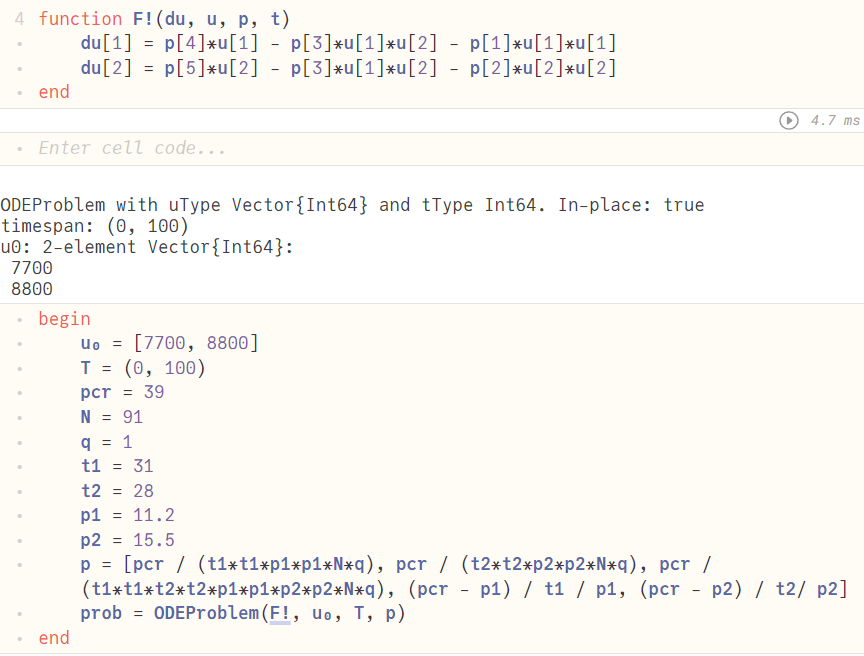
\includegraphics[width=0.7\textwidth,height=\textheight]{./tex2pdf.-eff22ba2c7041204/image/j1.PNG}
  \caption{Код для первой модели}\label{fig:001}
  }
  \end{figure}
\item
  Построим график изменения численности (fig.~\ref{fig:002})

  \begin{figure}
  \hypertarget{fig:002}{%
  \centering
  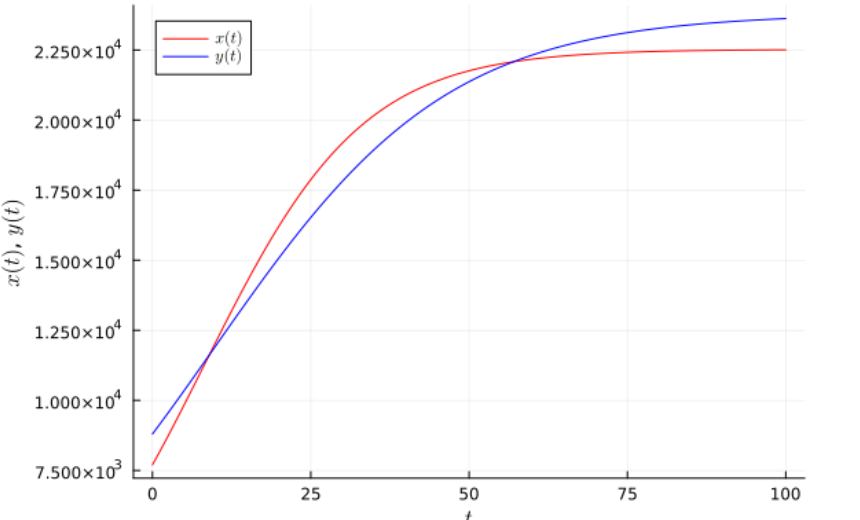
\includegraphics[width=0.7\textwidth,height=\textheight]{./tex2pdf.-eff22ba2c7041204/image/j1p.PNG}
  \caption{График для первой модели}\label{fig:002}
  }
  \end{figure}
\item
  Теперь зададим модель в Opemmodelica (fig.~\ref{fig:003}).

  \begin{figure}
  \hypertarget{fig:003}{%
  \centering
  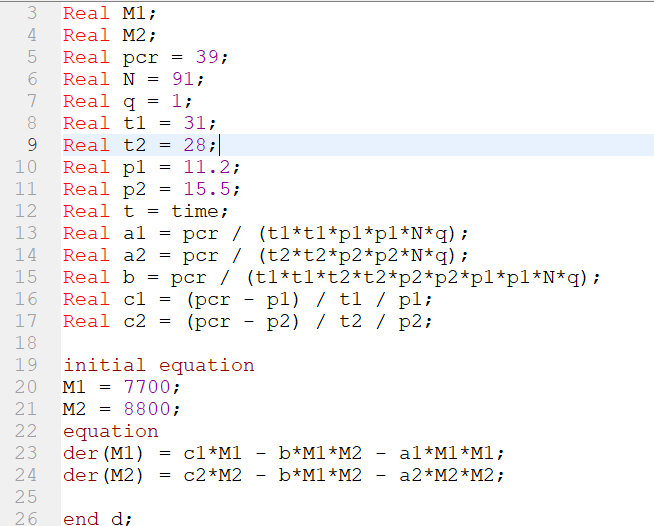
\includegraphics[width=0.7\textwidth,height=\textheight]{./tex2pdf.-eff22ba2c7041204/image/om1.PNG}
  \caption{Модель в openmodelica}\label{fig:003}
  }
  \end{figure}
\item
  Построим график (fig.~\ref{fig:004}).

  \begin{figure}
  \hypertarget{fig:004}{%
  \centering
  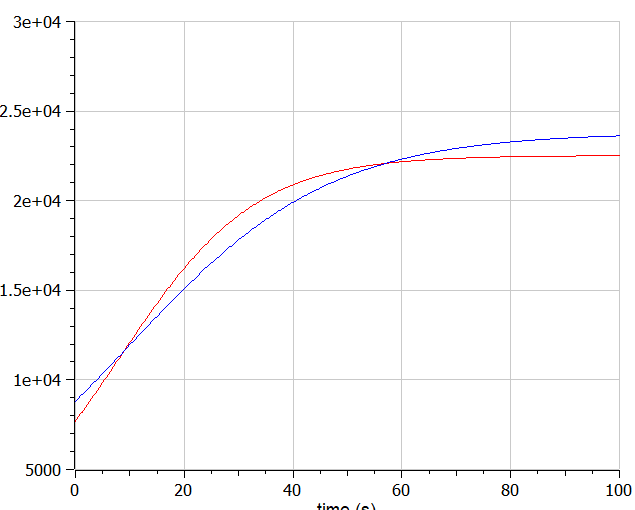
\includegraphics[width=0.7\textwidth,height=\textheight]{./tex2pdf.-eff22ba2c7041204/image/om1p.PNG}
  \caption{Результаты моделирования в openmodelica}\label{fig:004}
  }
  \end{figure}
\item
  Рассмотрим второй случай.
\item
  Система уравнений в Julia (fig.~\ref{fig:005}).

  \begin{figure}
  \hypertarget{fig:005}{%
  \centering
  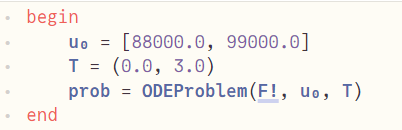
\includegraphics[width=0.7\textwidth,height=\textheight]{./tex2pdf.-eff22ba2c7041204/image/j2.PNG}
  \caption{Код для второй модели}\label{fig:005}
  }
  \end{figure}
\item
  Построим графики (fig.~\ref{fig:006})

  \begin{figure}
  \hypertarget{fig:006}{%
  \centering
  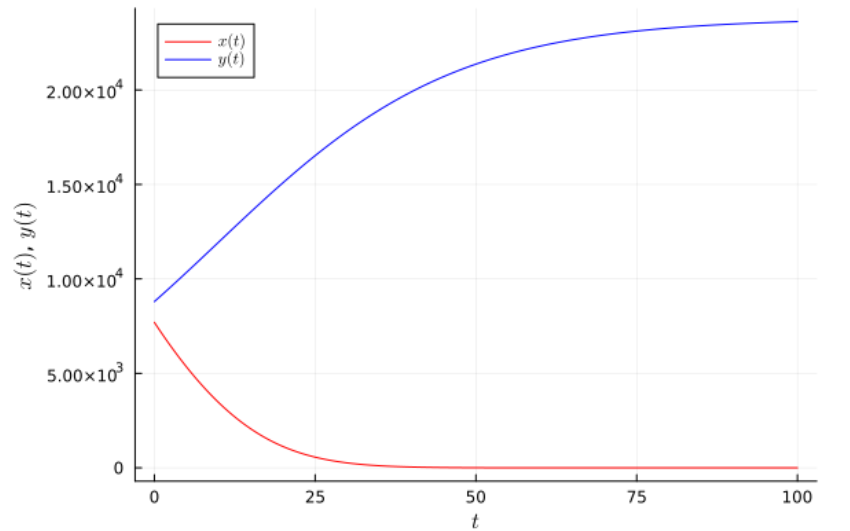
\includegraphics[width=0.7\textwidth,height=\textheight]{./tex2pdf.-eff22ba2c7041204/image/j2p.PNG}
  \caption{Результат моделирования в julia}\label{fig:006}
  }
  \end{figure}
\item
  Та же модель в openmodelica (fig.~\ref{fig:007})

  \begin{figure}
  \hypertarget{fig:007}{%
  \centering
  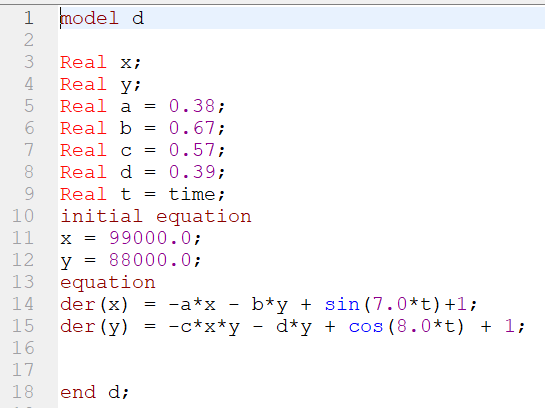
\includegraphics[width=0.7\textwidth,height=\textheight]{./tex2pdf.-eff22ba2c7041204/image/om2.PNG}
  \caption{Код для второй модели}\label{fig:007}
  }
  \end{figure}
\item
  И результаты моделирования (fig.~\ref{fig:008})

  \begin{figure}
  \hypertarget{fig:008}{%
  \centering
  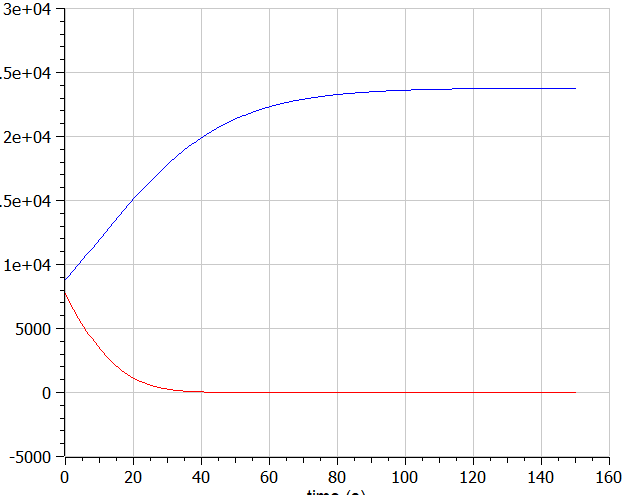
\includegraphics[width=0.7\textwidth,height=\textheight]{./tex2pdf.-eff22ba2c7041204/image/om2p.PNG}
  \caption{График модели}\label{fig:008}
  }
  \end{figure}
\end{enumerate}

\hypertarget{ux432ux44bux432ux43eux434ux44b}{%
\chapter{Выводы}\label{ux432ux44bux432ux43eux434ux44b}}

В итоге была рассмотрена простейшая модель конкуренции двух фирм . С
использованием Julia и OpenModelica построены графики изменения
численности, найдена точка максимума скорости.

\hypertarget{ux441ux43fux438ux441ux43eux43a-ux43bux438ux442ux435ux440ux430ux442ux443ux440ux44b}{%
\chapter*{Список
литературы}\label{ux441ux43fux438ux441ux43eux43a-ux43bux438ux442ux435ux440ux430ux442ux443ux440ux44b}}
\addcontentsline{toc}{chapter}{Список литературы}

\hypertarget{refs}{}
\begin{CSLReferences}{0}{0}
\leavevmode\vadjust pre{\hypertarget{ref-pres}{}}%
\CSLLeftMargin{1. }%
\CSLRightInline{Б. И. ГЕРАСИМОВ Д.Н.П. Н. П. ПУЧКОВ. {ДИФФЕРЕНЦИАЛЬНЫЕ
ДИНАМИЧЕСКИЕ МОДЕЛИ }. Издательство ГОУ ВПО ТГТУ, 2010.}

\leavevmode\vadjust pre{\hypertarget{ref-julia}{}}%
\CSLLeftMargin{2. }%
\CSLRightInline{В. В.О. {Основы численного анализа динамических систем}.
Новосибирск, ФИЦ ИВТ, 2022. 124 с.}

\end{CSLReferences}

\printbibliography

\end{document}
